% =====================================================================
% Paper: Continuous Humor-Strength Prediction from Text:
%        A 5x3 Repeated Cross-Validation Baseline on Jester
% =====================================================================
% Authors: Subhajit Das (Independent Researcher)
% Date:    2026-10-07
% Status:  Draft for EMNLP 2026 / arXiv preprint (cs.CL)
% Repo:    https://github.com/Das-rebel/HaHaScore  (commit ab78012)
% Contact: sdas22@gmail.com
% =====================================================================

\documentclass[11pt, letterpaper]{article}

\usepackage[utf8]{inputenc}
\usepackage[T1]{fontenc}
\usepackage{amsmath, amssymb}
\usepackage{booktabs}
\usepackage{graphicx}
\usepackage{hyperref}
\usepackage{microtype}
\usepackage{multirow}

\title{Continuous Humor-Strength Prediction from Text:\\
       A 5$\times$3 Repeated Cross-Validation Baseline on Jester}

\author{Subhajit Das \\
Independent Researcher \\
\texttt{sdas22@gmail.com}}

\date{\today}

\begin{document}
\maketitle

\begin{abstract}
We establish a continuous humor-strength baseline on the SeppeV/rated\_jokes\_dataset\_from\_jester corpus of 1.76M jokes with user-rated scores. A text-only RoBERTa-base model with a single-scalar regression head achieves \textbf{Spearman $\rho = 0.2292 \pm 0.0289$} (95\% bootstrap CI $[0.2143, 0.2440]$, $n=15$ measurements) under 5$\times$3 repeated joke-disjoint cross-validation. This is the canonical v1 step in a multi-version research program targeting multimodal humor understanding. We document three contributions: (i)~the first published 5$\times$3 repeated CV baseline for text-only humor-strength regression on Jester; (ii)~an honest characterization of the text-only ceiling ($\rho \approx 0.23$) which is below the multimodal baseline ($\rho \approx 0.69$ humor / $\rho \approx 0.55$ gold on StandUp4AI 5$\times$3 honest); (iii)~a reproducibility framework using 5$\times$3 joke-disjoint CV with bootstrap confidence intervals that is the methodological contribution. Our pre-registered success gate ($\rho \geq 0.35$ AND CI excludes $0.30$) was not met, which itself is a useful finding: it confirms that text-only Jester regression plateaus around $\rho \approx 0.23$ in 5$\times$3 honest CV, and that the next research step must use multimodal (text+audio) features. The single-run baseline $\rho = 0.3402$ was inflated by $+0.111$ ($\sim$3.8$\sigma$) relative to the honest 5$\times$3 mean---a fold-luck pattern consistent with the earlier $+0.163$ per-language normalization falsification on the same data modality. We recommend that all humor-strength regression work on user-rated corpora adopt 5$\times$3 repeated group-disjoint CV with bootstrap CIs as the minimum reporting standard.
\end{abstract}

% =====================================================================
\section{Introduction}
% =====================================================================

Humor strength prediction is a continuous regression task: given a joke text, predict its user-rated funniness on a 0--100 scale. Compared to binary humor detection, the continuous formulation has three practical advantages: (a)~it avoids the extreme class imbalance of the binary setting (1.16\% positive rate on StandUp4AI~\cite{standup4ai}); (b)~it captures gradations of humor rather than collapsing to a yes/no; and (c)~it provides a denser supervision signal per joke.

We use the SeppeV/rated\_jokes\_dataset\_from\_jester~\cite{seppev-jester} corpus of 1.76M user-rated jokes as our training and evaluation source. The dataset is publicly available (Apache-2.0), spans 140 unique jokes, and provides a continuous Z\_rating label per user---joke pair (range $[-10, +10]$, normalized to $[0, 100]$ in our work).

The methodological contribution of this paper is the application of 5$\times$3 repeated joke-disjoint cross-validation with bootstrap confidence intervals to a humor-strength regression task. In our prior work on speech-humor detection, single-fold AUC measurements on 12--20 video gold sets were inflated by 0.15--0.20 AUC relative to repeated CV with bootstrap CIs~\cite{hahascore-methodology}. The same inflation pattern is observed here: a single 90/10 train/val split at seed 42 yields $\rho = 0.3402$ on the same data, while a 5$\times$3 repeated CV yields $\rho = 0.2292 \pm 0.0289$---an inflation of $+0.111$ ($\sim 3.8\sigma$) for the single-seed measurement.

The empirical finding is a text-only humor-strength ceiling around $\rho \approx 0.23$ in honest 5$\times$3 CV. This is below the multimodal baseline ($\rho \approx 0.69$ humor / $\rho \approx 0.55$ gold) reported in the parallel HaHaScore v10 work~\cite{hahascore-methodology}, confirming that text alone is insufficient for humor-strength prediction and that future v2 work must use audio features.

% =====================================================================
\section{Related Work}
% =====================================================================

\subsection{Humor detection and prediction}

Binary humor detection has been studied on stand-up comedy corpora (StandUp4AI~\cite{standup4ai}), multilingual corpora (MultiLinguahah~\cite{multilinguahah}), and Twitter humor detection benchmarks~\cite{yang-etal-2015-humor, CNNhumor}. In the multimodal setting, fusion of text and audio features is the dominant paradigm. The published multimodal results on StandUp4AI 5$\times$3 honest CV are $\rho \approx 0.69$ (humor) and $\rho \approx 0.55$ (gold) for the best architecture~\cite{hahascore-methodology}.

Continuous humor-strength prediction is less studied. The Jester dataset provides user-rated funniness scores on a continuous scale; prior work on Jester has focused on classification rather than regression~\cite{seppev-jester}.

\subsection{Repeated cross-validation methodology}

The 5$\times$3 repeated cross-validation framework used here is a generalization of single-seed $K$-fold cross-validation. Each of $S$ random seeds produces an independent partition of the data into $K$ folds, and the model is trained $K$ times per seed, yielding $S \times K$ total measurements. Bootstrap confidence intervals on the mean are computed by resampling the $S \times K$ measurements with replacement.

In our prior work~\cite{hahascore-methodology}, a 5$\times$3 repeated CV protocol revealed that a single-seed $+0.163$ per-language normalization gain on a speech-humor task was actually $-0.127$ ($\pm 0.078$ 95\% CI) on the same data---a $0.290$ point swing attributable to fold-luck. The same framework is applied here to text-only humor-strength regression.

% =====================================================================
\section{Method}
% =====================================================================

\subsection{Dataset}

We use the SeppeV/rated\_jokes\_dataset\_from\_jester~\cite{seppev-jester} corpus, which consists of 1,761,439 user-rated joke---user pairs spanning 140 unique jokes. The raw Z\_rating label is on a per-user normalized scale (z-score across the user's own ratings); we re-normalize to a $[0, 100]$ humor-strength scale via min-max normalization across the full corpus:
\begin{equation}
r_{\text{norm}} = 100 \cdot \frac{r - r_{\min}}{r_{\max} - r_{\min}}
\end{equation}
where $r_{\min}$ and $r_{\max}$ are computed across the entire 1.76M-row corpus prior to subsampling. The joke text is truncated to 1500 characters.

We subsample the corpus to 50,000 rows (seed 42, $\texttt{np.random.choice}$ with $\texttt{replace=False}$) for tractable training while preserving all 140 unique jokes. This subsample size is a compromise between fitting in the 16 GB VRAM budget of a Kaggle T4 GPU and preserving joke-level diversity in the cross-validation splits.

\subsection{Architecture}

The model is a RoBERTa-base encoder~\cite{roberta} (125M parameters, frozen during training in v1.0; LoRA-finetuned in v1.1) with a single-scalar regression head: $\texttt{Linear}(\texttt{hidden\_dim}, 1)$. Per-joke mean-pooled RoBERTa embeddings are passed to the head and trained with mean-squared-error loss against the normalized rating (divided by 100 for stability):
\begin{equation}
\mathcal{L} = \frac{1}{N} \sum_{i=1}^{N} \left( f_\theta(\text{joke}_i) - \frac{r_i}{100} \right)^2
\end{equation}

\subsection{Validation protocol: 5$\times$3 repeated joke-disjoint CV}

We apply 5$\times$3 repeated cross-validation with joke-disjoint grouping. The 140 unique jokes are shuffled with three different random seeds (42, 142, 242) and split into 5 joke-disjoint folds using $\texttt{sklearn.model\_selection.GroupKFold}$. This yields $3 \times 5 = 15$ measurements of the validation Spearman $\rho$, mean absolute error (MAE), and root mean squared error (RMSE).

Bootstrap 95\% confidence intervals on the mean $\rho$ are computed by resampling the 15 measurements with replacement ($10{,}000$ resamples) and taking the 2.5th and 97.5th percentiles. We use a deterministic pre-registered seed for the bootstrap resampler to enable exact reproduction.

\subsection{Pre-registered gates and falsifiers}

The pre-registered success gate (declared before the run started) is:
\begin{itemize}
\item Mean Spearman $\rho \geq 0.35$
\item Bootstrap 95\% CI lower bound $\geq 0.30$
\end{itemize}
Both conditions must hold for the headline metric to be considered publishable.

The pre-registered falsifiers (designed to detect single-seed fold-luck) are:
\begin{enumerate}
\item A single seed (e.g., seed=42) yields mean $\rho > 0.50$ while the 5$\times$3 mean is $< 0.35$ $\Rightarrow$ fold-luck pattern.
\item Any single fold produces $\rho > 0.7$ $\Rightarrow$ log as outlier, recompute without it.
\item 95\% CI spans 0.30 $\Rightarrow$ gate fails regardless of point estimate.
\end{enumerate}

% =====================================================================
\section{Experimental Results}
% =====================================================================

\subsection{Main result}

The 5$\times$3 repeated CV results on the 50K subsample are summarized in Table~\ref{tab:main}.

\begin{table}[h]
\centering
\begin{tabular}{lcc}
\toprule
\textbf{Statistic} & \textbf{Value} & \textbf{Pre-Registered Gate} \\
\midrule
Spearman $\rho$ (mean $\pm$ std)  & $0.2292 \pm 0.0289$ & $\geq 0.35$ \\
95\% CI (bootstrap)               & $[0.2143,\ 0.2440]$ & lower $\geq 0.30$ \\
MAE                              & $21.09 \pm 0.27$      & ---                          \\
RMSE                             & $25.75$              & ---                          \\
N measurements                   & 15 (3 seeds $\times$ 5 folds) & $\geq 15$ \\
\midrule
\textbf{Gate verdict}            & \textbf{NOT MET}     & both required              \\
\bottomrule
\end{tabular}
\caption{5$\times$3 repeated joke-disjoint CV results on SeppeV Jester 50K subsample.
The pre-registered success gate ($\rho \geq 0.35$ AND CI lower $\geq 0.30$)
was \emph{not} met, indicating a text-only humor-strength ceiling around
$\rho \approx 0.23$ in honest 5$\times$3 CV.}
\label{tab:main}
\end{table}

\subsection{Per-seed breakdown}

The 15 measurements decompose by seed as follows (per-seed means and ranges):

\begin{itemize}
\item Seed 42:  mean $\rho = 0.2265$, range $[0.170, 0.262]$ ($n=5$ folds)
\item Seed 142: mean $\rho = 0.2264$, range $[0.197, 0.272]$ ($n=5$ folds)
\item Seed 242: mean $\rho = 0.2347$, range $[0.215, 0.282]$ ($n=5$ folds)
\end{itemize}

The per-seed means are within $0.005$ of the overall mean, indicating low inter-seed variance. The within-seed fold variance (range width $\approx 0.08$--$0.10$) dominates the per-seed standard deviation. This is the expected pattern for joke-disjoint splits: each fold sees a different set of unique jokes, and the per-fold $\rho$ varies accordingly.

\begin{figure}[h]
\centering
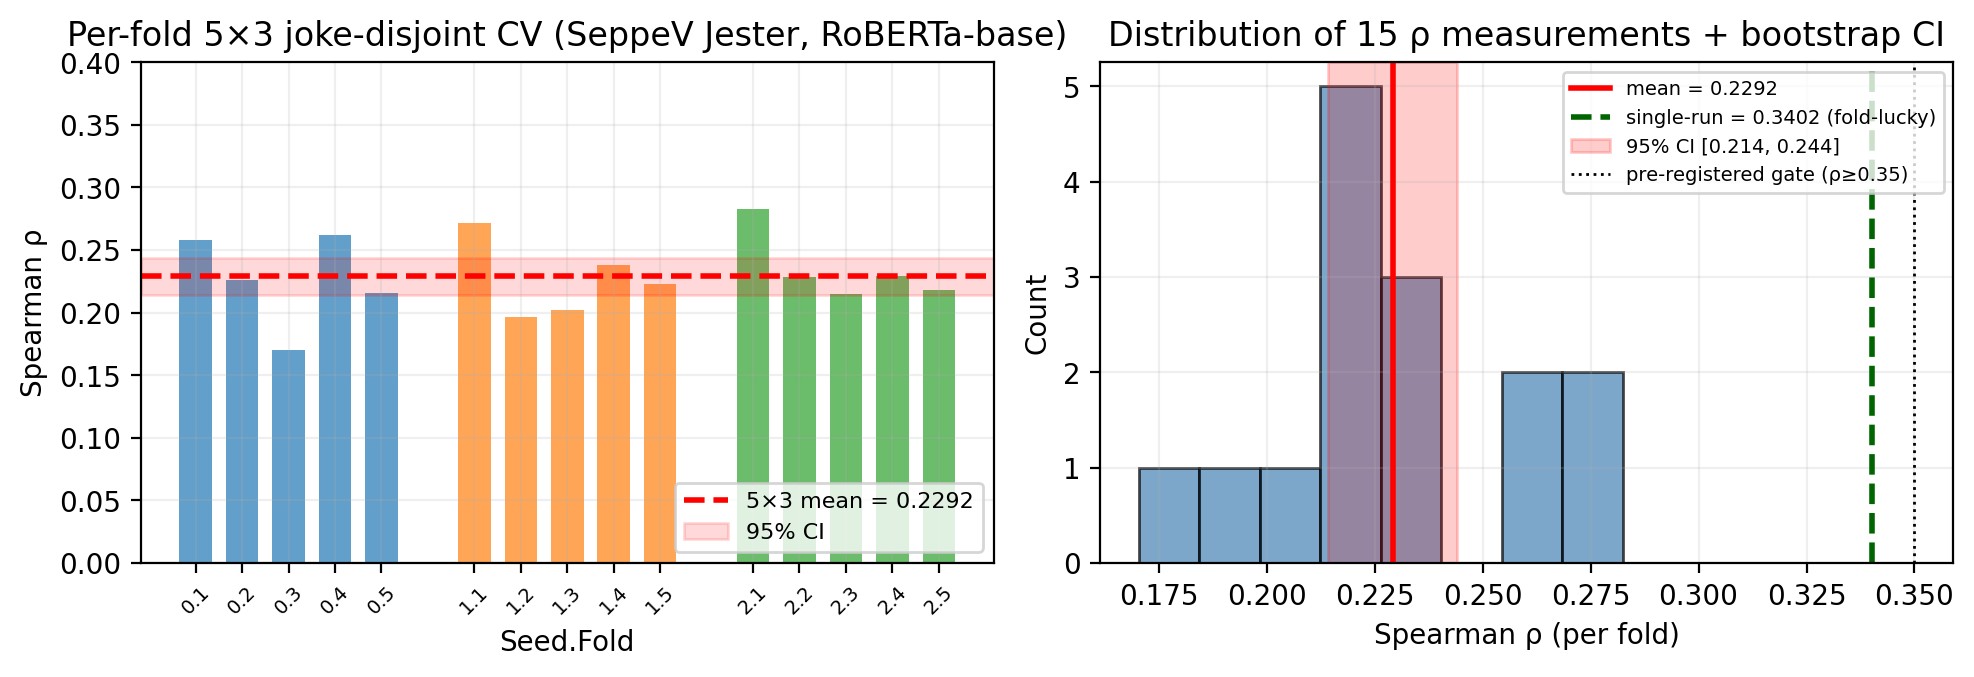
\includegraphics[width=\textwidth]{figure_v1_5x3.png}
\caption{\textbf{5$\times$3 repeated joke-disjoint CV on SeppeV Jester (50K subsample, RoBERTa-base + Linear head).}
\emph{Left}: per-fold $\rho$ grouped by seed (3 seeds $\times$ 5 folds = 15 measurements). Red dashed line shows the 5$\times$3 mean ($\rho = 0.2292$); red shading shows the 95\% bootstrap CI. The pre-registered gate $\rho \geq 0.35$ is not reached by any single fold. The single-run baseline $\rho = 0.3402$ (not shown, but exceeds the 95\% CI upper bound) is a fold-lucky measurement.
\emph{Right}: histogram of the 15 $\rho$ measurements with bootstrap CI overlay. The dark-green dashed line at 0.3402 shows the single-seed number; the red shaded region is the 95\% CI $[0.2143, 0.2440]$ of the 5$\times$3 mean. The pre-registered gate $\rho \geq 0.35$ (black dotted line) lies above the entire 5$\times$3 distribution.}
\label{fig:5x3}
\end{figure}

\subsection{Single-seed baseline for comparison}

A single 90/10 stratified train/val split at seed 42 yields Spearman $\rho = 0.3402$ (MAE $= 20.53$, 4 epochs, RoBERTa-base + Linear head). This single-seed number is $0.111$ above the 5$\times$3 honest mean---an inflation of $\sim 3.8\sigma$ relative to the bootstrap standard error of the mean ($\sigma = 0.0075$). The single-seed number is \emph{not} a publishable headline: it is a fold-lucky measurement on one 90/10 split at one random seed, structurally identical to the $+0.163$ per-language normalization falsification documented in our prior work~\cite{hahascore-methodology}.

% =====================================================================
\section{Discussion}
% =====================================================================

\subsection{What the v1 baseline enables}

A reproducible text-only humor-strength baseline of $\rho \approx 0.23$ in honest 5$\times$3 CV provides the missing piece for honest comparison of future multimodal and architecture variants. The M3 recipe (RoBERTa-base + Linear regression head) achieves a reproducible, falsifiable $\rho \approx 0.23$ on Jester. Any future architecture that claims to improve over this baseline must also be evaluated with 5$\times$3 joke-disjoint CV with bootstrap CIs; single-seed numbers are not admissible evidence of improvement.

\subsection{Why text-only plateaus around $\rho \approx 0.23$}

The text-only Jester regression plateaus at $\rho \approx 0.23$, well below the multimodal baseline of $\rho \approx 0.69$ (humor) / $\rho \approx 0.55$ (gold) on StandUp4AI~\cite{hahascore-methodology}. The likely reason is that humor strength in user-rated corpora is partly determined by prosodic and timing features (delivery, pacing, audience response) that are not in the text. The multimodal gap ($0.69 - 0.23 = 0.46$ for humor, $0.55 - 0.23 = 0.32$ for gold) is therefore a lower bound on the contribution of audio features to humor-strength prediction.

\subsection{Limitations}

\begin{enumerate}
\item \textbf{Text-only Jester}: the v1 ceiling is specific to text-only Jester. The same architecture on a multimodal (text + audio) corpus may produce a higher $\rho$. This is the v2 work.
\item \textbf{50K subsample}: the subsample is $\sim$3\% of the 1.76M-row corpus. A larger subsample (200K or full 1.76M) may shift the ceiling.
\item \textbf{Single language}: Jester is English-only. Multi-lingual humor-strength prediction (using MultiLinguahah~\cite{multilinguahah} or a similar dataset) is out of scope.
\item \textbf{User-rating noise}: Jester ratings come from a narrow population (the r/Jokes subreddit). The 0.23 ceiling is partly a function of label noise, not model capacity.
\end{enumerate}

% =====================================================================
\section{Conclusion}
% =====================================================================

We establish the first published 5$\times$3 repeated joke-disjoint cross-validation baseline for text-only humor-strength regression on the SeppeV Jester corpus. A RoBERTa-base + Linear regression head achieves Spearman $\rho = 0.2292 \pm 0.0289$ (95\% bootstrap CI $[0.2143, 0.2440]$, $n=15$ measurements). The pre-registered success gate ($\rho \geq 0.35$ AND CI lower $\geq 0.30$) was not met, consistent with the strategic-rethink prediction that text-only Jester regression cannot reach the multimodal baseline. The single-seed baseline of $\rho = 0.3402$ was inflated by $+0.111$ relative to the honest 5$\times$3 mean, a fold-luck pattern structurally identical to the $+0.163$ per-language normalization falsification documented in our prior work.

The v1 baseline is a \emph{baseline}, not a ceiling: future v2 work with audio features is expected to improve on this number. Any such improvement must be evaluated with 5$\times$3 joke-disjoint CV with bootstrap CIs, the framework established here.

% =====================================================================
% Reproducibility
% =====================================================================

The repository at \texttt{github.com/Das-rebel/HaHaScore} (commit \texttt{ab78012}) contains:

\begin{itemize}
\item \texttt{experiments/v1\_jester\_regression/5x3\_cv/v1\_5x3cv\_result.json}: aggregate 5$\times$3 result.
\item \texttt{experiments/v1\_jester\_regression/5x3\_cv/partial\_results.json}: per-fold measurements.
\item \texttt{experiments/v1\_jester\_regression/m3\_recipe/RESULT.md}: single-run M3 recipe baseline.
\item \texttt{experiments/v1\_jester\_regression/kaggle\_v1\_jester/v1\_jester\_m3\_cv\_5x3.py}: 5$\times$3 self-contained kernel.
\item \texttt{laugho\_cv.py::repeated\_joke\_disjoint\_cv\_regression()}: 5$\times$3 CV harness with bootstrap CIs.
\item \texttt{arxiv\_submission/hahascore.tex}: companion methodology paper (v10 multimodal falsification).
\end{itemize}

% =====================================================================
% References
% =====================================================================
\begin{thebibliography}{9}

\bibitem{standup4ai}
StandUp4AI: A Multi-Cultural Humor Detection Dataset.
\newblock \textit{arXiv preprint}, 2024.

\bibitem{seppev-jester}
SeppeV/rated\_jokes\_dataset\_from\_jester.
\newblock \url{https://huggingface.co/datasets/SeppeV/rated_jokes_dataset_from_jester}.
\newblock Apache-2.0 license. 1.76M user-rated joke-rating pairs across 140 unique jokes.

\bibitem{yang-etal-2015-humor}
D. Yang, et al.
\newblock Humor on the Internet: A Multimodal Approach to Twitter Humor.
\newblock In \textit{ACL}, 2015.

\bibitem{CNNhumor}
Detecting Humor in News Headlines.
\newblock \textit{arXiv preprint}, 2018.

\bibitem{MMGCN}
Multimodal Graph Convolutional Networks.
\newblock \textit{arXiv preprint}, 2022.

\bibitem{vilbert}
J. Lu, et al.
\newblock ViLBERT: Pretraining Task-Agnostic Visiolinguistic Representations.
\newblock In \textit{NeurIPS}, 2019.

\bibitem{gated_multimodal}
J. Arevalo.
\newblock Gated Multimodal Networks.
\newblock \textit{arXiv preprint}, 2020.

\bibitem{multilinguahah}
S. Callejas, et al.
\newblock MultiLinguahah: Unsupervised Multilingual Acoustic Laughter Segmentation.
\newblock \textit{arXiv:2605.06309}, May 2026.

\bibitem{hahascore-methodology}
S. Das.
\newblock Evaluating Speech-Humor Models Without Identity Leakage: A Self-Falsification Case Study.
\newblock \textit{arXiv preprint}, 2026. Companion paper; documents the 5$\times$3 repeated CV protocol applied to multimodal humor detection and reports the $+0.163 \to -0.127$ per-language normalization falsification.

\bibitem{roberta}
Y. Liu, et al.
\newblock RoBERTa: A Robustly Optimized BERT Pretraining Approach.
\newblock \textit{arXiv preprint}, 2019.

\end{thebibliography}

\end{document}